\chapter{Đặc Tả Yêu Cầu Phần Mềm}

% ============================================================
\section{Tổng Quan Sản Phẩm}
% ============================================================

\subsection{Mô Tả Hệ Thống}

\textbf{Tên hệ thống:} SmartDroneDelivery -- Nền tảng quản lý giao hàng bằng Drone tích hợp AI.

Hệ thống được xây dựng nhằm hỗ trợ doanh nghiệp logistics quản lý toàn bộ quy trình giao hàng
bằng máy bay không người lái (Drone), từ tiếp nhận yêu cầu giao hàng, quản lý khách hàng, kiện
hàng, trạm hạ cánh đến theo dõi trạng thái giao hàng theo thời gian thực và xác nhận hoàn tất.

\subsection{Các Thành Phần Hệ Thống}

Hệ thống gồm bốn thành phần chính:

\begin{itemize}
  \item \textbf{Website quản trị (Admin Web):} Dành cho Quản trị viên, Quản lý logistics,
        Điều phối viên và Nhân viên vận hành trạm. Cung cấp toàn bộ chức năng quản lý nghiệp vụ.
  \item \textbf{Giao diện Web cho người dùng cuối (Client Web):} Dành cho Khách hàng tạo đơn, theo dõi hành trình và Nhân viên vận hành trạm xác nhận đơn. Tương thích responsive tốt trên trình duyệt của các thiết bị di động.
  \item \textbf{RESTful API:} Phục vụ trao đổi dữ liệu giữa giao diện web quản trị và giao diện web người dùng cuối.
        và các dịch vụ bên ngoài.
  \item \textbf{Dịch vụ AI:} Hỗ trợ ước lượng thời gian giao hàng (ETA), chatbot trợ lý khách
        hàng và phân tích dữ liệu vận hành.
\end{itemize}

\subsection{Sơ Đồ Ngữ Cảnh Hệ Thống}

\begin{figure}[H]
  \centering
  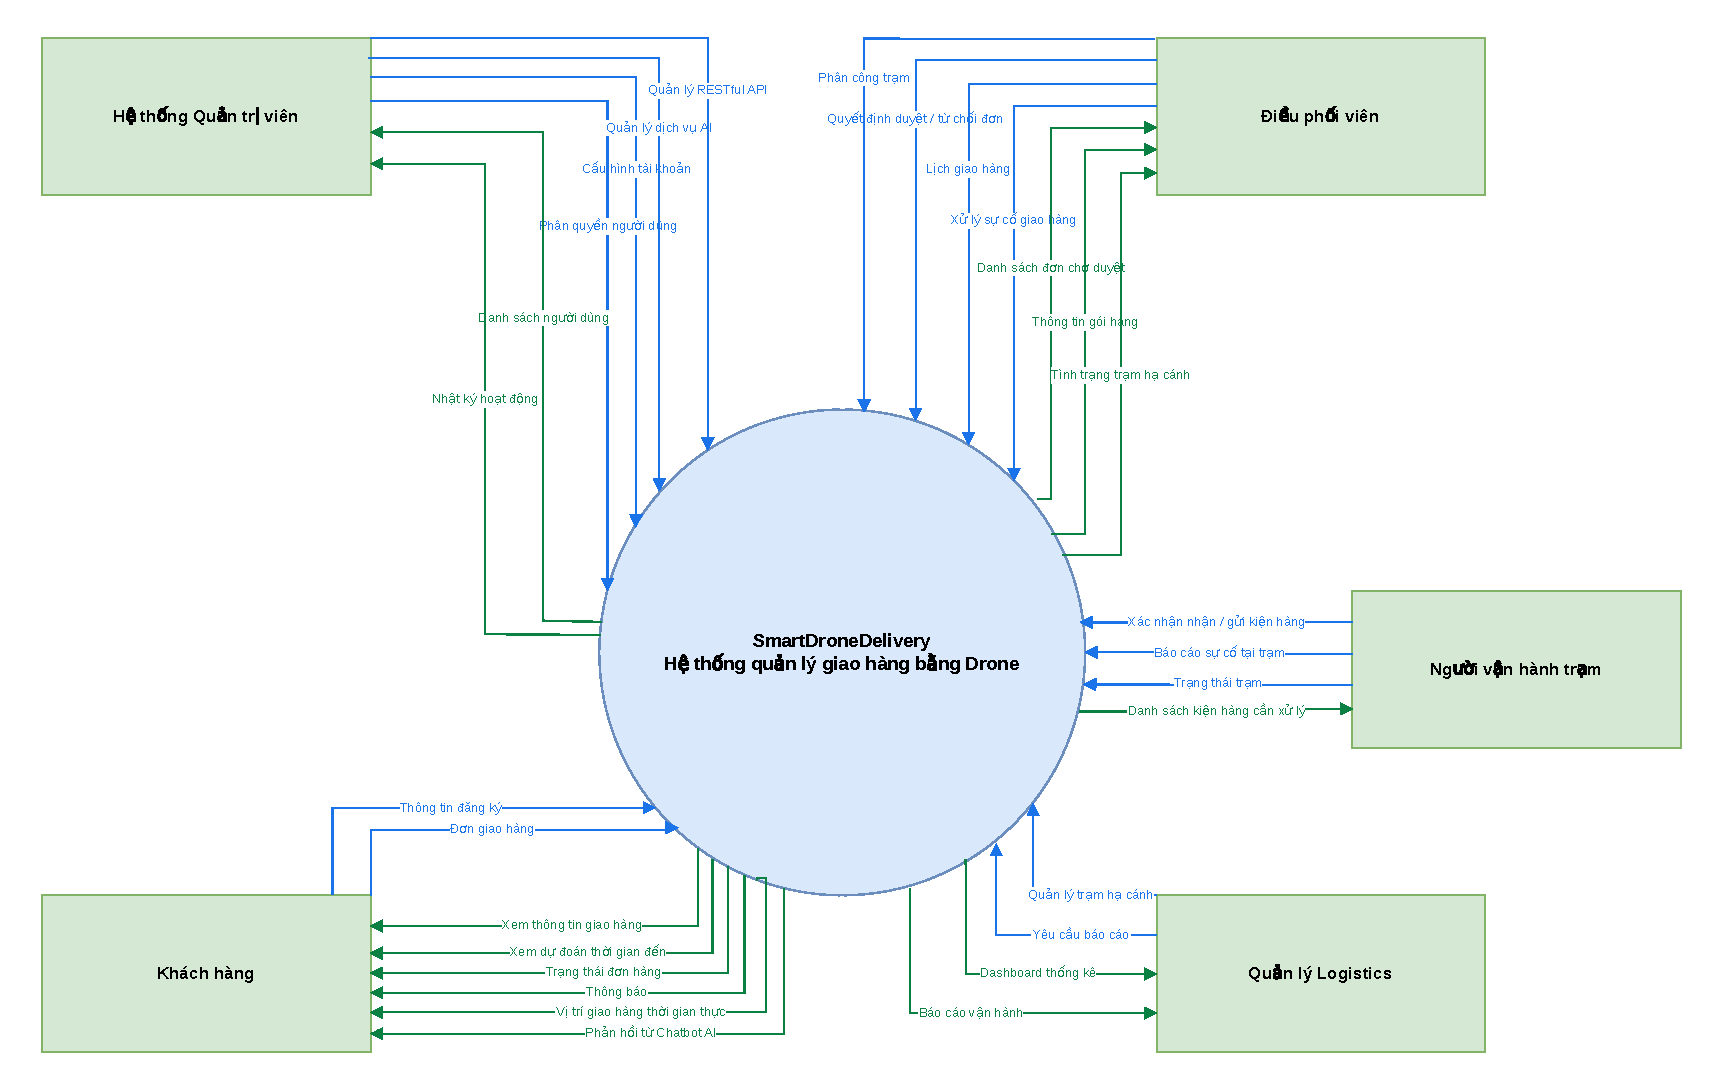
\includegraphics[width=0.85\textwidth]{so-do/context_diagram.pdf}
  \caption{Sơ đồ ngữ cảnh hệ thống SmartDroneDelivery}
  \label{fig:context-diagram}
\end{figure}

% ============================================================
\section{Yêu Cầu Người Dùng}
% ============================================================

\subsection{Các Tác Nhân Hệ Thống}

Hệ thống SmartDroneDelivery có năm tác nhân chính tương tác với hệ thống:

\begin{table}[H]
  \centering
  \begin{tabularx}{\textwidth}{|l|l|X|}
    \hline
    \textbf{Actor} & \textbf{Tên tiếng Việt} & \textbf{Mô tả vai trò} \\
    \hline
    Admin             & Quản trị viên              & Quản lý hệ thống, cấu hình, phân quyền người dùng và theo dõi nhật ký hoạt động \\ \hline
    Logistics Manager & Quản lý logistics          & Theo dõi báo cáo, thống kê, giám sát hiệu suất và đánh giá hoạt động giao hàng \\ \hline
    Dispatcher        & Điều phối viên             & Tiếp nhận, phê duyệt, lên lịch và điều phối đơn giao hàng; xử lý sự cố giao hàng thất bại \\ \hline
    Station Operator  & Nhân viên vận hành trạm    & Xác nhận kiện hàng tại trạm, cập nhật trạng thái và hỗ trợ xác nhận giao hàng thành công \\ \hline
    Customer          & Khách hàng                 & Đăng ký tài khoản, tạo đơn giao hàng, theo dõi tiến trình và xác nhận khi nhận hàng \\
    \hline
  \end{tabularx}
  \caption{Bảng các tác nhân hệ thống}
  \label{tab:actors}
\end{table}

\subsection{Sơ Đồ Use Case}

\clearpage
\subsubsection*{Use Case -- Quản Lý Khách Hàng Và Đơn Hàng Giao}

\begin{figure}[H]
  \centering
  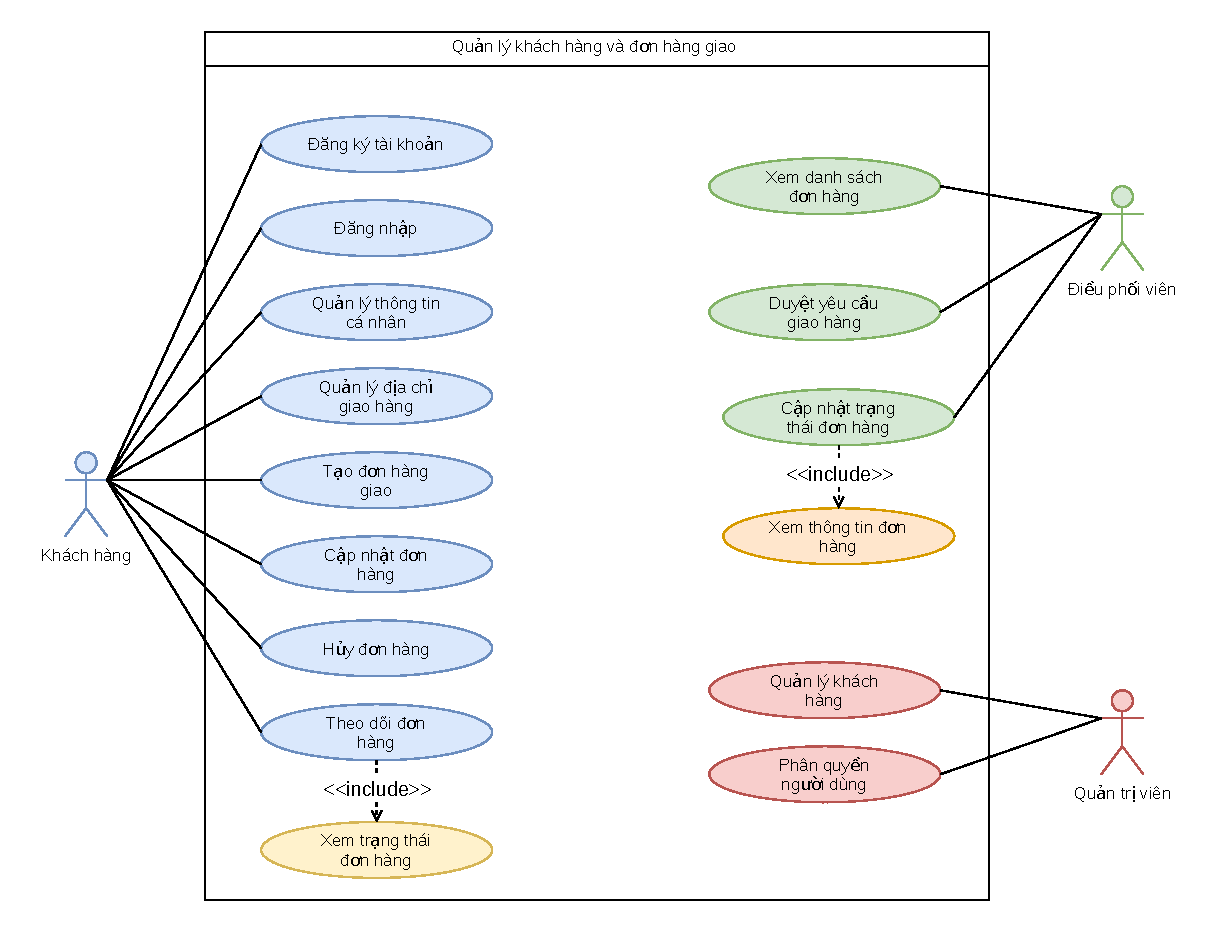
\includegraphics[width=0.88\textwidth]{so-do/uc_customer_order.pdf}
  \caption{Sơ đồ use case quản lý khách hàng và đơn hàng giao}
  \label{fig:uc-customer-order}
\end{figure}

\clearpage
\subsubsection*{Use Case -- Quản Lý Kiện Hàng}

\begin{figure}[H]
  \centering
  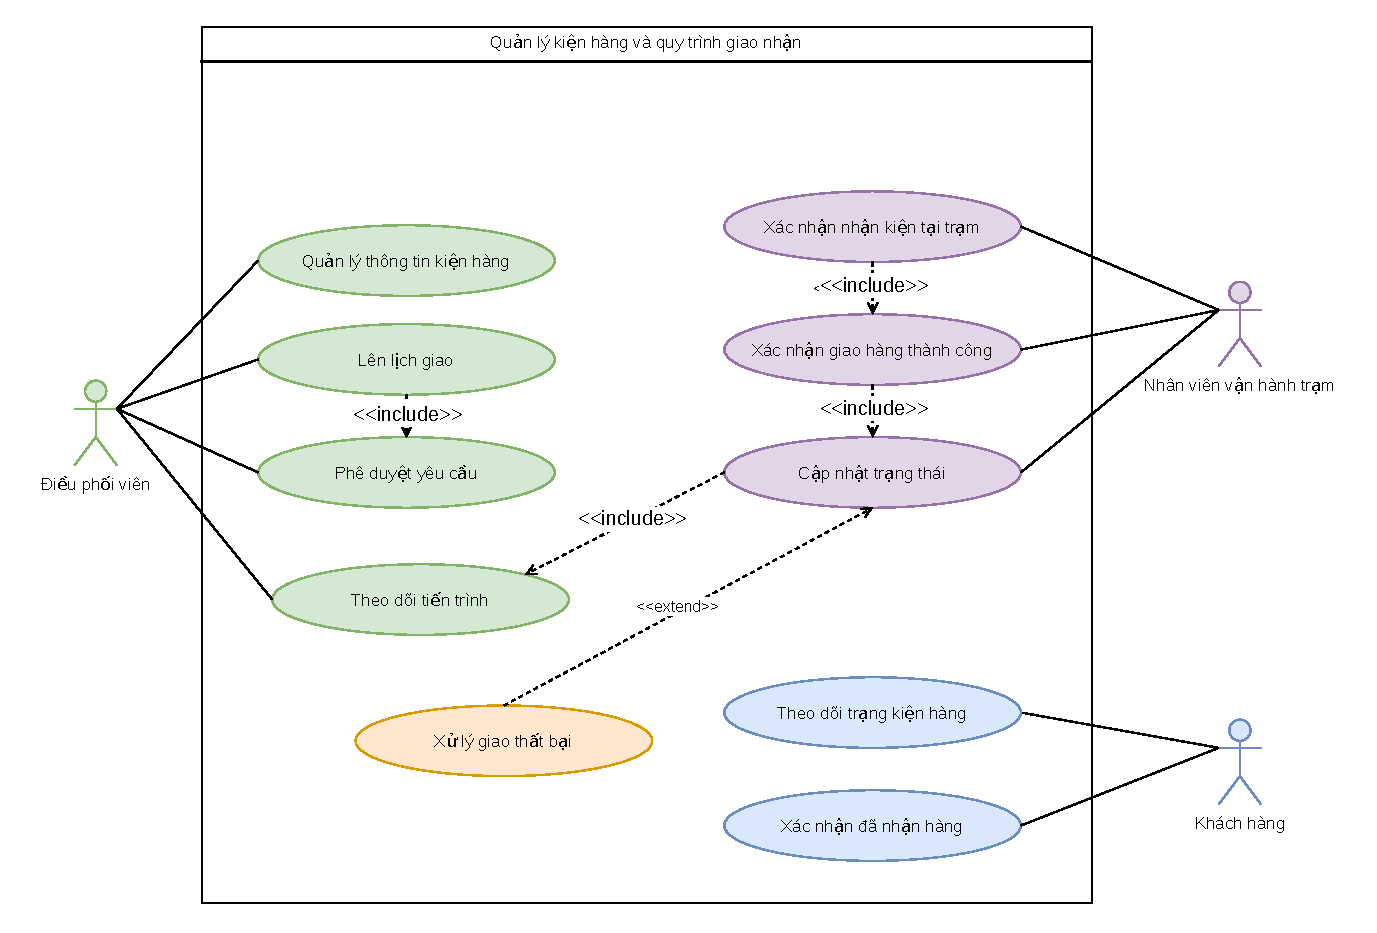
\includegraphics[width=0.88\textwidth]{so-do/uc_package_management.pdf}
  \caption{Sơ đồ use case quản lý kiện hàng}
  \label{fig:uc-package}
\end{figure}

\clearpage
\subsubsection*{Use Case -- Quản Lý Trạm Hạ Cánh}

\begin{figure}[H]
  \centering
  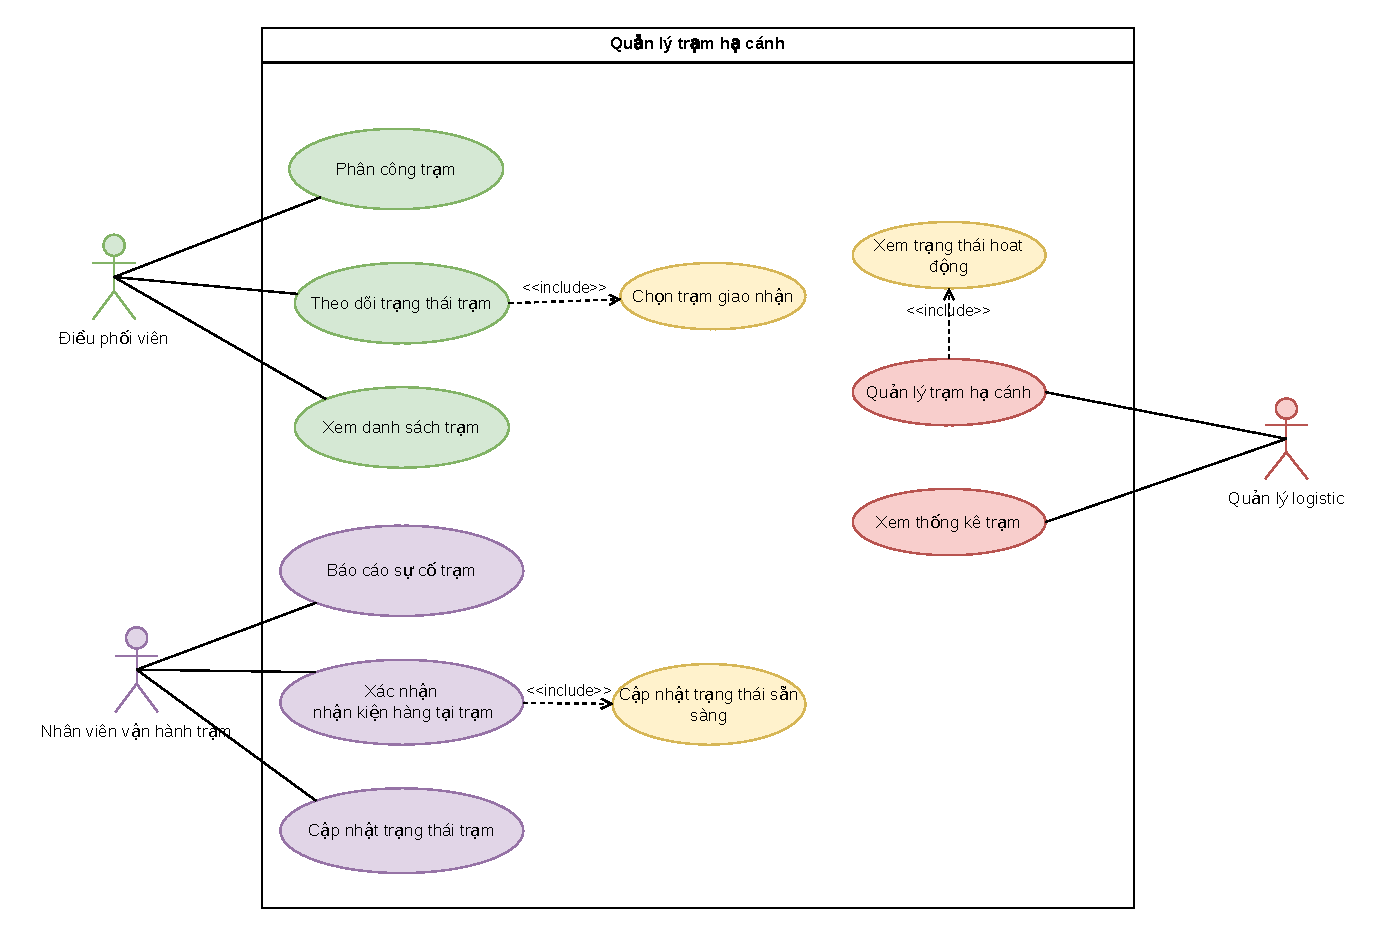
\includegraphics[width=0.88\textwidth]{so-do/uc_station_management.pdf}
  \caption{Sơ đồ use case quản lý trạm hạ cánh}
  \label{fig:uc-station}
\end{figure}

\clearpage
\subsubsection*{Use Case -- Theo Dõi Và Xác Nhận Giao Hàng}

\begin{figure}[H]
  \centering
  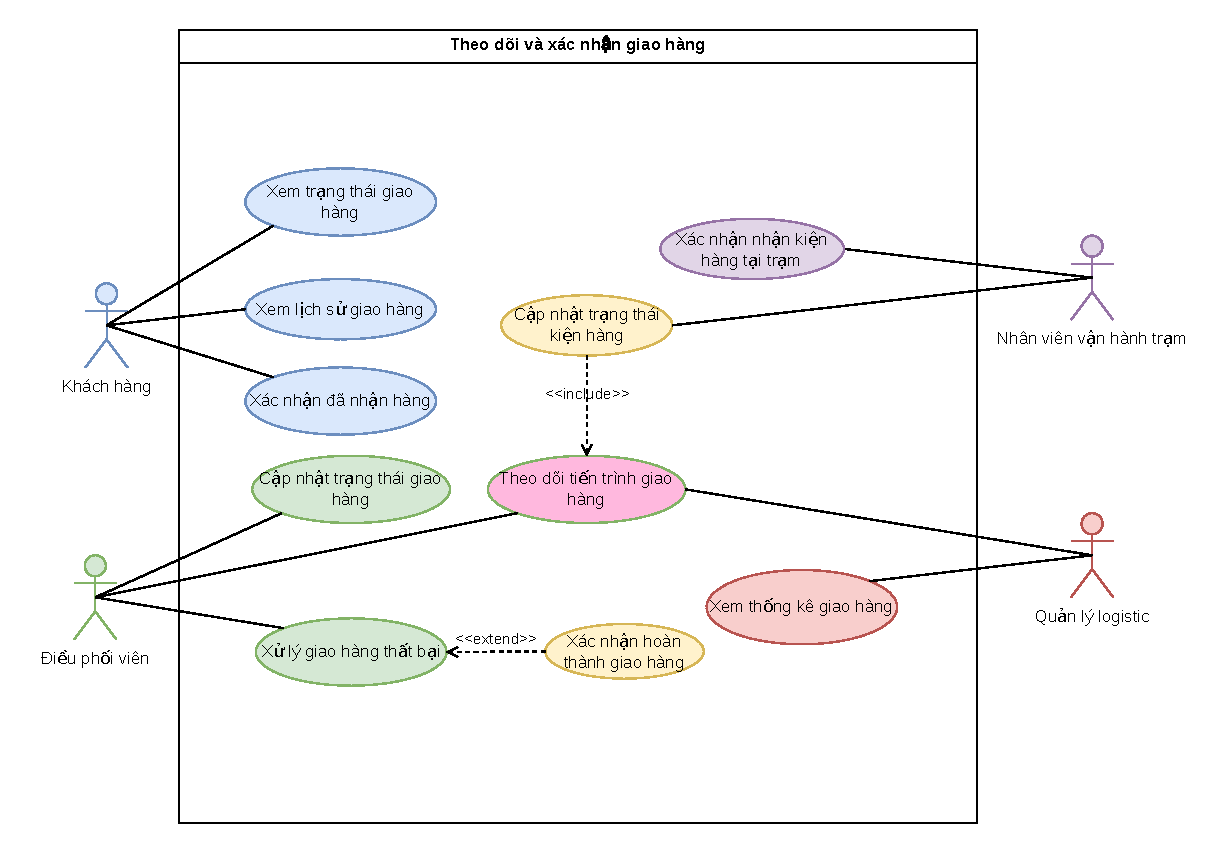
\includegraphics[width=0.88\textwidth]{so-do/uc_tracking_confirmation.pdf}
  \caption{Sơ đồ use case theo dõi và xác nhận giao hàng}
  \label{fig:uc-tracking}
\end{figure}

\clearpage
\subsubsection*{Use Case -- Phân Tích Và Dịch Vụ AI}

\begin{figure}[H]
  \centering
  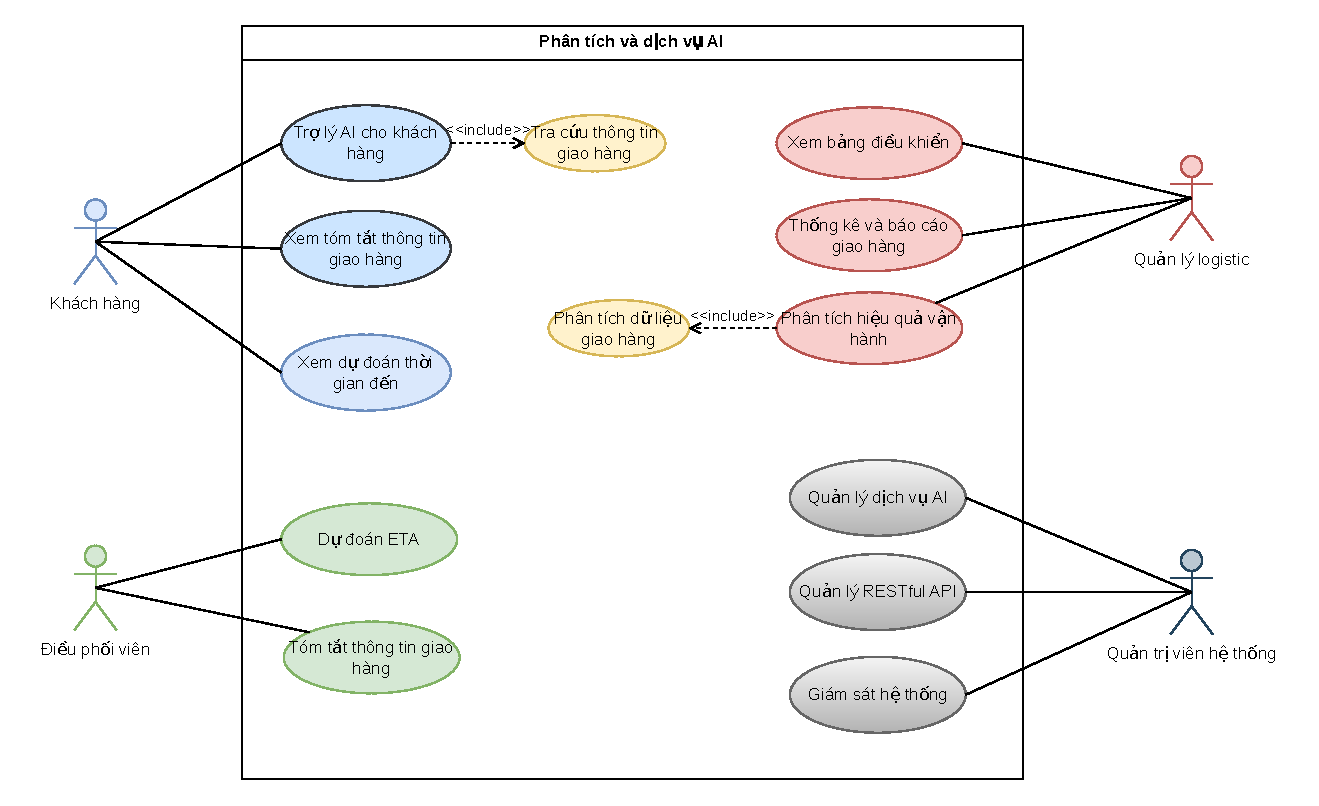
\includegraphics[width=0.88\textwidth]{so-do/uc_ai_analytics.pdf}
  \caption{Sơ đồ use case phân tích và dịch vụ AI}
  \label{fig:uc-ai}
\end{figure}

\subsection{Danh Sách Use Case Tổng Hợp}

\begin{table}[H]
  \centering
  \begin{tabularx}{\textwidth}{|l|X|l|}
    \hline
    \textbf{UC ID} & \textbf{Tên Use Case} & \textbf{Actor chính} \\
    \hline
    UC-01 & Đăng nhập \& Phân quyền                  & Tất cả \\ \hline
    UC-02 & Tạo đơn giao hàng mới                    & Customer \\ \hline
    UC-03 & Cập nhật / Hủy đơn giao hàng             & Customer \\ \hline
    UC-04 & Phê duyệt yêu cầu giao hàng              & Dispatcher \\ \hline
    UC-05 & Lập lịch giao hàng (Scheduling)           & Dispatcher \\ \hline
    UC-06 & Xử lý giao hàng thất bại                 & Dispatcher \\ \hline
    UC-07 & Xác nhận nhận/gửi kiện hàng tại trạm     & Station Operator \\ \hline
    UC-08 & Theo dõi giao hàng thời gian thực        & Customer, Dispatcher, Station Operator \\ \hline
    UC-09 & Xác nhận giao hàng thành công            & Station Operator, Customer \\ \hline
    UC-10 & Ước lượng thời gian giao hàng (ETA)      & Customer, Dispatcher \\ \hline
    UC-11 & Trợ lý AI cho khách hàng (Chatbot)       & Customer \\ \hline
    UC-12 & Tạo / Quản lý tài khoản người dùng       & Admin \\
    \hline
  \end{tabularx}
  \caption{Bảng tổng hợp use case hệ thống SmartDroneDelivery}
  \label{tab:usecases}
\end{table}

% ============================================================
\section{Đặc Tả Use Case}
% ============================================================

% --- UC-01 ---
\begin{table}[H]
  \centering
  \begin{tabularx}{\textwidth}{|l|X|}
    \hline
    \multicolumn{2}{|l|}{\textbf{UC-01: Đăng Nhập \& Phân Quyền}} \\
    \hline
    \textbf{Tác nhân}           & Tất cả actor (Customer, Dispatcher, Station Operator, Logistics Manager, Admin) \\ \hline
    \textbf{Mô tả}              & Người dùng đăng nhập vào hệ thống bằng tài khoản đã được cấp; hệ thống xác định vai trò và phân quyền tương ứng. \\ \hline
    \textbf{Điều kiện tiên quyết} & Người dùng đã có tài khoản hợp lệ trong hệ thống. \\ \hline
    \textbf{Luồng sự kiện chính} &
      \begin{enumerate}[leftmargin=*, nosep, topsep=0pt]
        \item Người dùng nhập email/tên đăng nhập và mật khẩu.
        \item Hệ thống xác thực thông tin đăng nhập.
        \item Hệ thống xác định vai trò (role) của tài khoản.
        \item Hệ thống chuyển hướng đến giao diện tương ứng với vai trò.
      \end{enumerate} \\ \hline
    \textbf{Luồng rẽ nhánh / Ngoại lệ} &
      \textbf{2a.} Sai tài khoản/mật khẩu $\rightarrow$ hệ thống báo lỗi, yêu cầu nhập lại.
      \newline
      \textbf{2b.} Tài khoản bị khóa $\rightarrow$ hệ thống thông báo không thể đăng nhập. \\ \hline
    \textbf{Hậu điều kiện}      & Người dùng được đăng nhập thành công, có phiên làm việc (session) hợp lệ. \\
    \hline
  \end{tabularx}
  \caption{Đặc tả UC-01: Đăng Nhập \& Phân Quyền}
  \label{tab:uc01}
\end{table}

% --- UC-02 ---
\begin{table}[H]
  \centering
  \begin{tabularx}{\textwidth}{|l|X|}
    \hline
    \multicolumn{2}{|l|}{\textbf{UC-02: Tạo Đơn Giao Hàng Mới}} \\
    \hline
    \textbf{Tác nhân}           & Khách hàng (Customer) \\ \hline
    \textbf{Mô tả}              & Khách hàng tạo một yêu cầu giao hàng mới trên hệ thống. \\ \hline
    \textbf{Điều kiện tiên quyết} & Đã đăng nhập; đã có ít nhất 1 địa chỉ giao hàng. \\ \hline
    \textbf{Luồng sự kiện chính} &
      \begin{enumerate}[leftmargin=*, nosep, topsep=0pt]
        \item Khách hàng chọn ``Tạo đơn hàng mới''.
        \item Nhập địa chỉ giao hàng, mô tả gói hàng, cân nặng, thời gian mong muốn.
        \item Hệ thống kiểm tra cân nặng gói hàng hợp lệ.
        \item Hệ thống tạo đơn hàng với trạng thái = ``Chờ duyệt''.
        \item Hệ thống thông báo cho Dispatcher về đơn hàng mới.
      \end{enumerate} \\ \hline
    \textbf{Luồng rẽ nhánh / Ngoại lệ} &
      \textbf{3a.} Gói hàng vượt tải trọng cho phép $\rightarrow$ báo lỗi, không tạo đơn.
      \newline
      \textbf{3b.} Địa chỉ ngoài vùng phục vụ $\rightarrow$ báo lỗi, không tạo đơn. \\ \hline
    \textbf{Hậu điều kiện}      & Đơn hàng mới được lưu vào hệ thống với trạng thái ``Chờ duyệt''. \\
    \hline
  \end{tabularx}
  \caption{Đặc tả UC-02: Tạo Đơn Giao Hàng Mới}
  \label{tab:uc02}
\end{table}

% --- UC-03 ---
\begin{table}[H]
  \centering
  \begin{tabularx}{\textwidth}{|l|X|}
    \hline
    \multicolumn{2}{|l|}{\textbf{UC-03: Cập Nhật / Hủy Đơn Giao Hàng}} \\
    \hline
    \textbf{Tác nhân}           & Khách hàng (Customer) \\ \hline
    \textbf{Mô tả}              & Khách hàng sửa thông tin hoặc hủy đơn khi đơn chưa được xử lý. \\ \hline
    \textbf{Điều kiện tiên quyết} & Đơn đang ở trạng thái ``Chờ duyệt'' (chưa gán trạm/drone). \\ \hline
    \textbf{Luồng sự kiện chính} &
      \begin{enumerate}[leftmargin=*, nosep, topsep=0pt]
        \item Khách hàng mở chi tiết đơn hàng.
        \item Chọn ``Sửa'' hoặc ``Hủy''.
        \item Nếu sửa: cập nhật lại thông tin, lưu thay đổi.
        \item Nếu hủy: xác nhận, hệ thống đổi trạng thái = ``Đã hủy''.
      \end{enumerate} \\ \hline
    \textbf{Luồng rẽ nhánh / Ngoại lệ} &
      \textbf{2a.} Đơn đã được duyệt/gán trạm $\rightarrow$ không cho sửa/hủy, báo ``Đơn đã xử lý, không thể thay đổi''. \\ \hline
    \textbf{Hậu điều kiện}      & Đơn được cập nhật hoặc chuyển trạng thái ``Đã hủy''. \\
    \hline
  \end{tabularx}
  \caption{Đặc tả UC-03: Cập Nhật / Hủy Đơn Giao Hàng}
  \label{tab:uc03}
\end{table}

% --- UC-04 ---
\begin{table}[H]
  \centering
  \begin{tabularx}{\textwidth}{|l|X|}
    \hline
    \multicolumn{2}{|l|}{\textbf{UC-04: Phê Duyệt Yêu Cầu Giao Hàng}} \\
    \hline
    \textbf{Tác nhân}           & Điều phối viên (Dispatcher) \\ \hline
    \textbf{Mô tả}              & Dispatcher xem xét và duyệt/từ chối đơn hàng mới. \\ \hline
    \textbf{Điều kiện tiên quyết} & Đơn đang ở trạng thái ``Chờ duyệt''. \\ \hline
    \textbf{Luồng sự kiện chính} &
      \begin{enumerate}[leftmargin=*, nosep, topsep=0pt]
        \item Dispatcher xem danh sách đơn ``Chờ duyệt''.
        \item Mở chi tiết đơn, kiểm tra thông tin gói hàng, địa chỉ.
        \item Bấm ``Duyệt'' $\rightarrow$ trạng thái chuyển ``Đã duyệt''.
        \item Hoặc bấm ``Từ chối'' $\rightarrow$ nhập lý do, trạng thái = ``Bị từ chối''.
      \end{enumerate} \\ \hline
    \textbf{Luồng rẽ nhánh / Ngoại lệ} &
      \textbf{3a.} Không có trạm hạ cánh khả dụng gần địa chỉ giao $\rightarrow$ hệ thống cảnh báo trước khi duyệt. \\ \hline
    \textbf{Hậu điều kiện}      & Đơn chuyển trạng thái ``Đã duyệt'' hoặc ``Bị từ chối''. \\
    \hline
  \end{tabularx}
  \caption{Đặc tả UC-04: Phê Duyệt Yêu Cầu Giao Hàng}
  \label{tab:uc04}
\end{table}

% --- UC-05 ---
\begin{table}[H]
  \centering
  \begin{tabularx}{\textwidth}{|l|X|}
    \hline
    \multicolumn{2}{|l|}{\textbf{UC-05: Lập Lịch Giao Hàng (Scheduling)}} \\
    \hline
    \textbf{Tác nhân}           & Điều phối viên (Dispatcher) \\ \hline
    \textbf{Mô tả}              & Dispatcher xếp lịch giao hàng cho đơn đã duyệt, gán trạm và thời gian dự kiến. \\ \hline
    \textbf{Điều kiện tiên quyết} & Đơn đang ở trạng thái ``Đã duyệt''. \\ \hline
    \textbf{Luồng sự kiện chính} &
      \begin{enumerate}[leftmargin=*, nosep, topsep=0pt]
        \item Dispatcher chọn đơn đã duyệt.
        \item Hệ thống gợi ý trạm hạ cánh gần địa chỉ giao (đang hoạt động).
        \item Dispatcher chọn trạm và thời gian giao dự kiến.
        \item Hệ thống cập nhật trạng thái đơn = ``Đã lên lịch''.
      \end{enumerate} \\ \hline
    \textbf{Luồng rẽ nhánh / Ngoại lệ} &
      \textbf{2a.} Không có trạm khả dụng $\rightarrow$ hệ thống báo, Dispatcher phải chọn trạm khác hoặc hoãn lịch. \\ \hline
    \textbf{Hậu điều kiện}      & Đơn được gán trạm và thời gian giao, trạng thái ``Đã lên lịch''. \\
    \hline
  \end{tabularx}
  \caption{Đặc tả UC-05: Lập Lịch Giao Hàng}
  \label{tab:uc05}
\end{table}

% --- UC-06 ---
\begin{table}[H]
  \centering
  \begin{tabularx}{\textwidth}{|l|X|}
    \hline
    \multicolumn{2}{|l|}{\textbf{UC-06: Xử Lý Giao Hàng Thất Bại}} \\
    \hline
    \textbf{Tác nhân}           & Điều phối viên (Dispatcher) \\ \hline
    \textbf{Mô tả}              & Dispatcher xử lý các đơn hàng giao không thành công (extend từ UC-08 Theo dõi tiến trình giao hàng). \\ \hline
    \textbf{Điều kiện tiên quyết} & Đơn đang ở trạng thái ``Đang giao'' và phát sinh sự cố. \\ \hline
    \textbf{Luồng sự kiện chính} &
      \begin{enumerate}[leftmargin=*, nosep, topsep=0pt]
        \item Hệ thống / Station Operator ghi nhận sự cố giao hàng.
        \item Dispatcher xem chi tiết sự cố.
        \item Dispatcher quyết định: giao lại, hủy đơn, hoặc liên hệ khách hàng.
        \item Hệ thống cập nhật trạng thái đơn tương ứng.
      \end{enumerate} \\ \hline
    \textbf{Luồng rẽ nhánh / Ngoại lệ} &
      \textbf{3a.} Sự cố nghiêm trọng (mất kiện hàng) $\rightarrow$ chuyển cho Logistics Manager xử lý thêm. \\ \hline
    \textbf{Hậu điều kiện}      & Đơn được xử lý lại hoặc chuyển trạng thái ``Giao thất bại''. \\
    \hline
  \end{tabularx}
  \caption{Đặc tả UC-06: Xử Lý Giao Hàng Thất Bại}
  \label{tab:uc06}
\end{table}

% --- UC-07 ---
\begin{table}[H]
  \centering
  \begin{tabularx}{\textwidth}{|l|X|}
    \hline
    \multicolumn{2}{|l|}{\textbf{UC-07: Xác Nhận Nhận/Gửi Kiện Hàng Tại Trạm}} \\
    \hline
    \textbf{Tác nhân}           & Nhân viên vận hành trạm (Station Operator) \\ \hline
    \textbf{Mô tả}              & Nhân viên trạm xác nhận đã nhận kiện hàng từ khách hoặc đặt kiện hàng lên drone để giao. \\ \hline
    \textbf{Điều kiện tiên quyết} & Đơn đã được lên lịch, gán đúng trạm này. \\ \hline
    \textbf{Luồng sự kiện chính} &
      \begin{enumerate}[leftmargin=*, nosep, topsep=0pt]
        \item Nhân viên trạm nhận kiện hàng (từ khách hàng hoặc từ kho).
        \item Quét/nhập mã đơn hàng để xác nhận.
        \item Hệ thống cập nhật trạng thái kiện hàng = ``Đã nhận tại trạm''.
        \item Khi drone sẵn sàng, nhân viên xác nhận gửi đi, trạng thái = ``Đang giao''.
      \end{enumerate} \\ \hline
    \textbf{Luồng rẽ nhánh / Ngoại lệ} &
      \textbf{2a.} Kiện hàng không khớp mã đơn $\rightarrow$ báo lỗi, không xác nhận. \\ \hline
    \textbf{Hậu điều kiện}      & Trạng thái kiện hàng được cập nhật đúng theo bước xử lý tại trạm. \\
    \hline
  \end{tabularx}
  \caption{Đặc tả UC-07: Xác Nhận Nhận/Gửi Kiện Hàng Tại Trạm}
  \label{tab:uc07}
\end{table}

% --- UC-08 ---
\begin{table}[H]
  \centering
  \begin{tabularx}{\textwidth}{|l|X|}
    \hline
    \multicolumn{2}{|l|}{\textbf{UC-08: Theo Dõi Giao Hàng Thời Gian Thực}} \\
    \hline
    \textbf{Tác nhân}           & Khách hàng, Điều phối viên, Nhân viên vận hành trạm \\ \hline
    \textbf{Mô tả}              & Xem vị trí và trạng thái di chuyển của đơn hàng đang giao, cập nhật theo thời gian thực. \\ \hline
    \textbf{Điều kiện tiên quyết} & Đơn đang ở trạng thái ``Đang giao''. \\ \hline
    \textbf{Luồng sự kiện chính} &
      \begin{enumerate}[leftmargin=*, nosep, topsep=0pt]
        \item Actor mở màn hình theo dõi đơn hàng.
        \item Hệ thống lấy tọa độ mới nhất qua Supabase Realtime.
        \item Bản đồ cập nhật vị trí di chuyển liên tục.
        \item Khi đơn hoàn tất, dừng cập nhật vị trí.
      \end{enumerate} \\ \hline
    \textbf{Luồng rẽ nhánh / Ngoại lệ} &
      \textbf{2a.} Mất kết nối dữ liệu vị trí $\rightarrow$ hiển thị trạng thái cuối cùng ghi nhận được, báo ``Đang chờ cập nhật''. \\ \hline
    \textbf{Hậu điều kiện}      & Actor xem được vị trí/trạng thái giao hàng mới nhất. \\
    \hline
  \end{tabularx}
  \caption{Đặc tả UC-08: Theo Dõi Giao Hàng Thời Gian Thực}
  \label{tab:uc08}
\end{table}

% --- UC-09 ---
\begin{table}[H]
  \centering
  \begin{tabularx}{\textwidth}{|l|X|}
    \hline
    \multicolumn{2}{|l|}{\textbf{UC-09: Xác Nhận Giao Hàng Thành Công}} \\
    \hline
    \textbf{Tác nhân}           & Nhân viên vận hành trạm, Khách hàng \\ \hline
    \textbf{Mô tả}              & Xác nhận đơn hàng đã được giao đến tay người nhận. \\ \hline
    \textbf{Điều kiện tiên quyết} & Drone đã đến điểm giao (đơn ở trạng thái ``Đang giao'', gần hoàn tất). \\ \hline
    \textbf{Luồng sự kiện chính} &
      \begin{enumerate}[leftmargin=*, nosep, topsep=0pt]
        \item Nhân viên trạm hoặc Khách hàng xác nhận đã nhận được kiện hàng.
        \item Hệ thống cập nhật trạng thái đơn = ``Đã giao thành công''.
        \item Hệ thống gửi thông báo hoàn tất cho Khách hàng.
      \end{enumerate} \\ \hline
    \textbf{Luồng rẽ nhánh / Ngoại lệ} &
      \textbf{1a.} Không xác nhận trong thời gian quy định $\rightarrow$ hệ thống tự động nhắc nhở hoặc chuyển trạng thái ``Chờ xác nhận quá hạn''. \\ \hline
    \textbf{Hậu điều kiện}      & Đơn hàng ở trạng thái ``Đã giao thành công'', quy trình giao hàng kết thúc. \\
    \hline
  \end{tabularx}
  \caption{Đặc tả UC-09: Xác Nhận Giao Hàng Thành Công}
  \label{tab:uc09}
\end{table}

% --- UC-10 ---
\begin{table}[H]
  \centering
  \begin{tabularx}{\textwidth}{|l|X|}
    \hline
    \multicolumn{2}{|l|}{\textbf{UC-10: Ước Lượng Thời Gian Giao Hàng (ETA)}} \\
    \hline
    \textbf{Tác nhân}           & Khách hàng, Điều phối viên \\ \hline
    \textbf{Mô tả}              & Hệ thống ước tính thời gian dự kiến giao hàng dựa trên khoảng cách và tốc độ trung bình (heuristic). \\ \hline
    \textbf{Điều kiện tiên quyết} & Đơn đã được lên lịch, có tọa độ trạm xuất phát và địa chỉ giao. \\ \hline
    \textbf{Luồng sự kiện chính} &
      \begin{enumerate}[leftmargin=*, nosep, topsep=0pt]
        \item Hệ thống lấy tọa độ trạm và địa chỉ giao.
        \item Tính khoảng cách và áp dụng công thức ước lượng tốc độ trung bình.
        \item Hiển thị ETA cho Khách hàng/Dispatcher.
        \item ETA được cập nhật lại khi có thay đổi vị trí thực tế.
      \end{enumerate} \\ \hline
    \textbf{Luồng rẽ nhánh / Ngoại lệ} &
      \textbf{1a.} Thiếu dữ liệu tọa độ $\rightarrow$ hiển thị ``Chưa thể ước lượng''. \\ \hline
    \textbf{Hậu điều kiện}      & Actor xem được thời gian dự kiến giao hàng. \\
    \hline
  \end{tabularx}
  \caption{Đặc tả UC-10: Ước Lượng Thời Gian Giao Hàng}
  \label{tab:uc10}
\end{table}

% --- UC-11 ---
\begin{table}[H]
  \centering
  \begin{tabularx}{\textwidth}{|l|X|}
    \hline
    \multicolumn{2}{|l|}{\textbf{UC-11: Trợ Lý AI Cho Khách Hàng (Chatbot)}} \\
    \hline
    \textbf{Tác nhân}           & Khách hàng \\ \hline
    \textbf{Mô tả}              & Khách hàng đặt câu hỏi liên quan đến đơn hàng; chatbot dựa trên LLM API trả lời tự động (include: Tra cứu thông tin giao hàng). \\ \hline
    \textbf{Điều kiện tiên quyết} & Khách hàng đã đăng nhập. \\ \hline
    \textbf{Luồng sự kiện chính} &
      \begin{enumerate}[leftmargin=*, nosep, topsep=0pt]
        \item Khách hàng mở khung chat, nhập câu hỏi.
        \item Hệ thống gửi câu hỏi kèm ngữ cảnh đơn hàng đến LLM API.
        \item Hệ thống tra cứu thông tin đơn hàng liên quan nếu cần.
        \item Chatbot trả lời câu hỏi của khách hàng.
      \end{enumerate} \\ \hline
    \textbf{Luồng rẽ nhánh / Ngoại lệ} &
      \textbf{2a.} LLM API không phản hồi/lỗi $\rightarrow$ hiển thị ``Chatbot tạm thời không khả dụng'', gợi ý liên hệ Dispatcher. \\ \hline
    \textbf{Hậu điều kiện}      & Khách hàng nhận được câu trả lời liên quan đến đơn hàng. \\
    \hline
  \end{tabularx}
  \caption{Đặc tả UC-11: Trợ Lý AI Cho Khách Hàng}
  \label{tab:uc11}
\end{table}

% --- UC-12 ---
\begin{table}[H]
  \centering
  \begin{tabularx}{\textwidth}{|l|X|}
    \hline
    \multicolumn{2}{|l|}{\textbf{UC-12: Tạo / Quản Lý Tài Khoản Người Dùng}} \\
    \hline
    \textbf{Tác nhân}           & Quản trị viên hệ thống (Admin) \\ \hline
    \textbf{Mô tả}              & Admin tạo, chỉnh sửa, phân quyền tài khoản cho các actor trong hệ thống. \\ \hline
    \textbf{Điều kiện tiên quyết} & Admin đã đăng nhập với quyền quản trị. \\ \hline
    \textbf{Luồng sự kiện chính} &
      \begin{enumerate}[leftmargin=*, nosep, topsep=0pt]
        \item Admin mở màn hình quản lý người dùng.
        \item Tạo tài khoản mới, gán vai trò (Customer / Dispatcher / Station Operator / Logistics Manager / Admin).
        \item Hoặc chỉnh sửa/khóa tài khoản hiện có.
        \item Hệ thống lưu thay đổi và ghi log hoạt động.
      \end{enumerate} \\ \hline
    \textbf{Luồng rẽ nhánh / Ngoại lệ} &
      \textbf{2a.} Email/tài khoản đã tồn tại $\rightarrow$ báo lỗi, yêu cầu nhập lại. \\ \hline
    \textbf{Hậu điều kiện}      & Tài khoản được tạo/cập nhật, có hiệu lực ngay trong hệ thống. \\
    \hline
  \end{tabularx}
  \caption{Đặc tả UC-12: Tạo / Quản Lý Tài Khoản Người Dùng}
  \label{tab:uc12}
\end{table}

% ============================================================
\section{Yêu Cầu Chức Năng}
% ============================================================

\subsection{Tổng Quan Chức Năng Hệ Thống}

Hệ thống SmartDroneDelivery được tổ chức thành bốn nhóm chức năng chính:

\begin{itemize}
  \item \textbf{Quản lý tài khoản và phân quyền:} Đăng nhập, đăng ký, quản lý người dùng theo vai trò.
  \item \textbf{Quản lý đơn hàng và kiện hàng:} Tạo, duyệt, lên lịch, theo dõi và xác nhận giao hàng.
  \item \textbf{Quản lý trạm hạ cánh:} Thêm, sửa, xóa trạm; cập nhật trạng thái hoạt động.
  \item \textbf{Dịch vụ AI hỗ trợ:} Ước lượng ETA và chatbot trợ lý khách hàng.
\end{itemize}

\subsection{Danh Sách Yêu Cầu Chức Năng}

\subsubsection{FR-01: Đăng Nhập Hệ Thống}
\textbf{Mô tả:} Cho phép tất cả người dùng đăng nhập vào hệ thống theo tài khoản được cấp.

\textbf{Chức năng:}
\begin{itemize}
  \item Nhập email/tên đăng nhập và mật khẩu.
  \item Xác thực tài khoản, cấp phiên làm việc (JWT token).
  \item Phân quyền và điều hướng đến giao diện theo vai trò.
  \item Hỗ trợ đăng xuất khỏi hệ thống.
\end{itemize}

\subsubsection{FR-02: Quản Lý Tài Khoản Người Dùng}
\textbf{Mô tả:} Admin quản lý toàn bộ tài khoản trong hệ thống.

\textbf{Chức năng:}
\begin{itemize}
  \item Tạo tài khoản mới với vai trò tương ứng.
  \item Chỉnh sửa thông tin tài khoản.
  \item Khóa/mở khóa tài khoản.
  \item Ghi log hoạt động quản trị.
\end{itemize}

\subsubsection{FR-03: Quản Lý Đơn Giao Hàng}
\textbf{Mô tả:} Cho phép Khách hàng tạo, theo dõi và quản lý đơn giao hàng; Dispatcher phê duyệt và lên lịch.

\textbf{Chức năng:}
\begin{itemize}
  \item Tạo đơn giao hàng mới với thông tin gói hàng và địa chỉ.
  \item Cập nhật hoặc hủy đơn (khi đơn chưa được xử lý).
  \item Phê duyệt hoặc từ chối đơn (Dispatcher).
  \item Lập lịch giao hàng, gán trạm hạ cánh (Dispatcher).
  \item Xử lý đơn giao thất bại.
\end{itemize}

\subsubsection{FR-04: Quản Lý Kiện Hàng Tại Trạm}
\textbf{Mô tả:} Nhân viên trạm xác nhận và cập nhật trạng thái kiện hàng trong quá trình vận chuyển.

\textbf{Chức năng:}
\begin{itemize}
  \item Quét/nhập mã đơn để xác nhận nhận kiện hàng.
  \item Cập nhật trạng thái kiện hàng (Đã nhận tại trạm, Đang giao).
  \item Xác nhận giao hàng thành công.
\end{itemize}

\subsubsection{FR-05: Quản Lý Trạm Hạ Cánh}
\textbf{Mô tả:} Quản lý thông tin và trạng thái các trạm hạ cánh của drone trong hệ thống.

\textbf{Chức năng:}
\begin{itemize}
  \item Thêm trạm hạ cánh mới (tên, tọa độ, sức chứa).
  \item Cập nhật thông tin trạm.
  \item Xóa trạm.
  \item Cập nhật trạng thái hoạt động (Đang hoạt động / Bảo trì / Ngừng).
\end{itemize}

\subsubsection{FR-06: Theo Dõi Giao Hàng Thời Gian Thực}
\textbf{Mô tả:} Cho phép Khách hàng, Dispatcher và Nhân viên trạm theo dõi vị trí và trạng thái giao hàng.

\textbf{Chức năng:}
\begin{itemize}
  \item Hiển thị bản đồ theo dõi vị trí drone theo thời gian thực.
  \item Cập nhật trạng thái đơn liên tục qua Supabase Realtime.
  \item Hiển thị ETA (thời gian dự kiến giao hàng).
\end{itemize}

\subsubsection{FR-07: Dịch Vụ Ước Lượng ETA}
\textbf{Mô tả:} Hệ thống tự động tính toán thời gian dự kiến giao hàng dựa trên tọa độ và tốc độ trung bình.

\textbf{Chức năng:}
\begin{itemize}
  \item Tính khoảng cách từ trạm đến địa chỉ giao hàng.
  \item Áp dụng công thức ước lượng ETA theo tốc độ trung bình drone.
  \item Cập nhật ETA theo vị trí thực tế khi đơn đang giao.
\end{itemize}

\subsubsection{FR-08: Chatbot Trợ Lý AI}
\textbf{Mô tả:} Chatbot hỗ trợ Khách hàng trả lời câu hỏi liên quan đến đơn hàng thông qua LLM API.

\textbf{Chức năng:}
\begin{itemize}
  \item Giao diện chat trực tiếp trong ứng dụng.
  \item Tích hợp LLM API (Anthropic/OpenAI) xử lý ngôn ngữ tự nhiên.
  \item Tra cứu thông tin đơn hàng ngữ cảnh để trả lời chính xác.
  \item Fallback: thông báo lỗi và gợi ý liên hệ Dispatcher khi API không khả dụng.
\end{itemize}

% ============================================================
\section{Yêu Cầu Phi Chức Năng}
% ============================================================

\subsection{Xác Thực và Phân Quyền}
\begin{itemize}
  \item Hệ thống phải hỗ trợ cơ chế đăng nhập an toàn cho tất cả người dùng.
  \item Phân quyền dựa trên vai trò (RBAC) cho các nhóm người dùng: Khách hàng, Điều phối viên, Nhân viên vận hành trạm, Quản lý logistics, Quản trị viên hệ thống.
  \item Các thao tác nhạy cảm (xóa đơn hàng, thay đổi trạng thái giao hàng) chỉ được thực hiện bởi người dùng có quyền hạn tương ứng.
\end{itemize}

\subsection{Thời Gian Phản Hồi}
\begin{itemize}
  \item Thời gian phản hồi cho các thao tác thông dụng (tạo đơn, xem trạng thái) phải dưới 3 giây.
  \item Các giao dịch quan trọng (xác nhận giao hàng, cập nhật trạng thái drone) phải hoàn tất trong vòng 10 giây.
\end{itemize}

\subsection{Hỗ Trợ Người Dùng (Khả Năng Tải)}
\begin{itemize}
  \item Hệ thống phải hỗ trợ tối thiểu 100 người dùng đồng thời (CCU) với hiệu suất ổn định và không làm giảm khả năng xử lý.
  \item Kiến trúc hệ thống phải cho phép mở rộng dễ dàng (scalability) khi số lượng người dùng và đơn hàng tăng lên.
\end{itemize}

\subsection{RESTful API Phục Vụ Tích Hợp Bên Ngoài}
\begin{itemize}
  \item Cung cấp API chuẩn RESTful để tích hợp với các hệ thống logistics, kho vận hoặc dịch vụ bên ngoài.
  \item API phải có tài liệu hướng dẫn và đặc tả đầy đủ (Swagger/OpenAPI).
\end{itemize}

\subsection{Triển Khai Bằng Supabase}
\begin{itemize}
  \item Hệ thống phải được triển khai và quản lý trên nền tảng Supabase để đảm bảo tính linh hoạt và dễ bảo trì.
  \item Supabase hỗ trợ cơ sở dữ liệu PostgreSQL, xác thực người dùng (Auth) và API tích hợp, giúp giảm tải cấu hình thủ công.
\end{itemize}

\subsection{Sự Linh Hoạt (Khả Năng Tương Thích)}
\begin{itemize}
  \item Giao diện Web phải tương thích tốt với nhiều loại thiết bị và độ phân giải màn hình khác nhau (Responsive Design cho cả máy tính, máy tính bảng và điện thoại di động).
  \item Thiết kế giao diện phải thân thiện, trực quan, dễ sử dụng cho mọi nhóm người dùng.
\end{itemize}

\subsection{Giám Sát Hệ Thống, Kiểm Toán và Sao Lưu}
\begin{itemize}
  \item Hệ thống phải có cơ chế giám sát thời gian thực (real-time monitoring) cho drone, trạm hạ cánh và tiến trình giao hàng.
  \item Ghi nhật ký kiểm toán (audit logging) chi tiết cho mọi thao tác quan trọng trên hệ thống.
  \item Hỗ trợ cơ chế sao lưu dữ liệu (backup) định kỳ và khôi phục (restore) nhanh chóng khi xảy ra sự cố.
\end{itemize}

\subsection{Kiến Trúc Phần Mềm và Khả Năng Bảo Trì}
\begin{itemize}
  \item Kiến trúc phần mềm phải được thiết kế theo dạng module hóa, tách biệt rõ ràng giữa các thành phần hệ thống.
  \item Đảm bảo mã nguồn dễ bảo trì, nâng cấp và mở rộng tính năng mới khi có nhu cầu trong tương lai.
\end{itemize}

% ============================================================
\section{Phụ Lục Yêu Cầu}
% ============================================================

\subsection{Quy Tắc Nghiệp Vụ}

\begin{longtable}{|l|p{12cm}|}
  \hline
  \textbf{Mã} & \textbf{Mô tả quy tắc} \\
  \hline
  \endhead
  \hline
  \endfoot
  BR-01 & Cân nặng gói hàng tối đa là 5kg; vượt quá không được tạo đơn. \\ \hline
  BR-02 & Khách hàng chỉ được hủy/sửa đơn khi đơn ở trạng thái ``Chờ duyệt''. \\ \hline
  BR-03 & Mỗi đơn hàng chỉ được gán một trạm hạ cánh tại một thời điểm. \\ \hline
  BR-04 & Trạm đang trong trạng thái ``Bảo trì'' hoặc ``Ngừng'' không được gán đơn hàng mới. \\ \hline
  BR-05 & Mật khẩu tối thiểu 8 ký tự, gồm chữ hoa, chữ thường và số. \\ \hline
  BR-06 & Mỗi tài khoản chỉ được đăng nhập đồng thời trên một thiết bị (session duy nhất). \\ \hline
  BR-07 & Hệ thống tự động cập nhật ETA mỗi 30 giây khi đơn đang trong trạng thái ``Đang giao''. \\ \hline
  BR-08 & Sau 24 giờ không xác nhận giao hàng, hệ thống tự động chuyển sang ``Chờ xác nhận quá hạn''. \\
\end{longtable}

\subsection{Yêu Cầu Chung}

\begin{itemize}
  \item Hệ thống phải hoạt động ổn định trên nền tảng Web, hỗ trợ hiển thị responsive mượt mà trên các thiết bị di động (iOS và Android) thông qua trình duyệt.
  \item Giao diện hỗ trợ đầy đủ tiếng Việt; các thông báo lỗi hiển thị rõ ràng bằng tiếng Việt.
  \item Dữ liệu nhạy cảm (mật khẩu, thông tin khách hàng) phải được mã hóa và không lưu dưới dạng plain text.
  \item Mọi API endpoint phải yêu cầu xác thực JWT; tài nguyên không có token hợp lệ sẽ bị từ chối (\texttt{401 Unauthorized}).
  \item Hệ thống phải có cơ chế ghi log mọi thao tác quan trọng (tạo/sửa/xóa đơn, thay đổi trạng thái kiện hàng, quản lý tài khoản).
  \item Thư thông báo được gửi qua email hoặc push notification khi trạng thái đơn hàng thay đổi.
  \item Hệ thống phải tuân thủ GDPR cơ bản: không chia sế dữ liệu cá nhân khách hàng cho bên thứ ba không được ủy quyền.
\end{itemize}

\subsection{Danh Sách Thông Báo Hệ Thống}

\begin{longtable}{|l|l|p{9cm}|}
  \hline
  \textbf{Mã} & \textbf{Loại} & \textbf{Nội dung thông báo} \\
  \hline
  \endhead
  \hline
  \endfoot
  MSG-001 & Thành công  & Đơn hàng đã được tạo thành công. \\ \hline
  MSG-002 & Thành công  & Đơn hàng đã được phê duyệt. \\ \hline
  MSG-003 & Thành công  & Đơn hàng đã được giao thành công. \\ \hline
  MSG-004 & Lỗi         & Sai tài khoản hoặc mật khẩu. Vui lòng thử lại. \\ \hline
  MSG-005 & Lỗi         & Tài khoản đã bị khóa. Vui lòng liên hệ quản trị viên. \\ \hline
  MSG-006 & Lỗi         & Gói hàng vượt tải trọng cho phép (tối đa 5kg). \\ \hline
  MSG-007 & Lỗi         & Địa chỉ giao hàng nằm ngoài vùng phục vụ. \\ \hline
  MSG-008 & Lỗi         & Không có trạm hạ cánh khả dụng trong khu vực. \\ \hline
  MSG-009 & Cảnh báo    & Đơn hàng đã được xử lý, không thể thay đổi. \\ \hline
  MSG-010 & Cảnh báo    & Chatbot tạm thời không khả dụng. Vui lòng liên hệ điều phối viên. \\ \hline
  MSG-011 & Thông tin   & Phiên làm việc sắp hết hạn (5 phút). \\ \hline
  MSG-012 & Thông tin   & Đơn hàng của bạn đang được giao. ETA: \textit{[thời gian ước lượng]}. \\
\end{longtable}
